\chapter{基于进化算法的FPGA脉动阵列快速硬核布局方法}

本章详细介绍本文的布局问题建模,NSGA-II和CMA-ES的算法原理,RapidLayout框架流程与实现细节。首先介绍了
面向 UltraScale+ FPGA 的布局问题建模,明确了问题的优化目标与限制;其次讨论了本文的创新基因型设计与相应的
解合法化过程;然后阐述了NSGA-II与CMA-ES的算法原理与实现方案;最终介绍了RapidLayout布局框架的工作流,并
以层层递进的方式举例阐述了脉动阵列的布局实现过程。

\section{问题建模}

本文将FPGA硬核布局建模为一个存在约束的多目标优化问题。首先,本文以Xilinx UltraScale+ VU11P FPGA举例说明异构FPGA中硬核的排布方法和
架构带来的布局约束条件,建立布局问题的背景;然后说明本文中布局问题的多个优化目标,以及根据优化目标和约束条件建立布局模型的方法。

图\ref{fig:architecture}展示了Xilinx UltraScale+系列VU11P FPGA的整体架构和放大后两个时钟域内部的硬核排布。首先,VU11P FPGA
由3个超逻辑域(Super Logic Region, SLR)构成,每个超逻辑域内的可编程器件构成和排布完全相同;其次,超逻辑域内包含三种硬核,分别是
DSP48E2, RAMB18, URAM288,每种硬核按列排布,但不同硬核列之间的分布却是无规则的;同时,三种硬核的大小不同:URAM288最大,RAMB18其次,
而DSP48E2最小。VU11P共有960个URAM288单元、4032个RAMB18单元,9216个DSP48单元,因此硬核的资源是不均衡的。
硬核列之间排布的不规则、硬核资源的不均衡和硬核大小本身的不同给布局带来了挑战:低质量的排布会造成部分计算单元内部连线过长,
导致整体设计时钟频率低,且可布线程度(Routability)降低导致布线失败。
另一方面,由于硬核之间为级联设计了专用的高速布线资源,所以硬核的布局存在约束:
\begin{itemize}
    \item 级联的硬核必须按从下(South)到上(North)的顺序排布,且不能跨超逻辑域(SLR)。
    \item 级联的DSP48E2与URAM288必须映射在相邻的两个Site上。
    \item 级联的RAMB18必须映射在距离1个Site的相邻两个位置上。
\end{itemize}


\begin{figure}[h]
	\centering
	\includegraphics[width=\textwidth]{figure/architecture}
	\caption{Xilinx UltraScale+ VU11P 硬核列分布示意图} 
	\label{fig:architecture}
\end{figure}

FPGA布局的目的一般有两个:将Technology Mapping并分组后的逻辑网表映射到FPGA的物理器件上,保证设计可以布线;另一个目的是在可布线
的基础上追求小的延迟(delay),也就是尽可能短的关键路径(Critical Path)和尽可能高的时钟频率。因此,我们将硬核布局问题建立为一个
有约束的多目标优化问题:


\begin{equation} \label{eq:obj1}
	min \sum_{i,j} ((\Delta{x_{i,j}} + \Delta{y_{i,j}}) \cdot w_{i,j})^2 
\end{equation}

\begin{equation} \label{eq:obj2}
	 \min (\max_{k} BBoxSize(C_k))
\end{equation}

subject to:

% rectangle region bound
\begin{equation} \label{eq:region}
  0 \leq x_i,y_i < XMAX,YMAX
\end{equation}


% no overlap
\begin{equation} \label{eq:overlap}
    {x_i,y_i} \neq {x_j,y_j}
\end{equation}

% cascade connection placement requirement
\begin{equation} \label{eq:cascade}
  \begin{aligned}[b]
	& \textrm{if } i \textrm{ is cascaded after } j \textrm{ in the same column: }
  x_i = x_j \\
	& y_i =
	\begin{cases}
		 y_j + 1  & i, j \in \{  DSP, URAM  \} \\
		 y_j + 2  & i, j \in \{  RAMB \}
	\end{cases}
\end{aligned}
\end{equation}

在以上的等式中:
\begin{itemize}
	\item $i \in \{ DSP, RAM, URAM \} $ 表示逻辑网表映射到的FPGA上物理硬核单元。
	\item $C_k$ 表示卷积计算单元 $k$,其中包含2个URAM,18个DSP和8个BRAM。 
	\item $\Delta{x_{i,j}} + \Delta{y_{i,j}}$ 表示硬核$i$与硬核$j$之间的曼哈顿距离(Manhattan Distance)。
	\item $w_{i,j}$ 表示硬核$i$与硬核$j$之间距离的权重,这里我们用两个硬核之间连线的数目作为权重。
	\item $BBoxSize()$ 表示卷积核$C_k$的Bounding Box限制框尺寸,也就是限制框宽与高的和. 
	\item $x_i$ and $y_i$ 表示硬核$i$的RPM绝对坐标~\cite{ug903},用于计算两硬核之间的距离和卷积计算单元的限制框尺寸.
\end{itemize}

\subsection{布局问题的目标函数}
我们用线长的平方来表征布局的阻塞性能,如式\ref{eq:obj1},用最大限制框(Bounding Box)尺寸来表征卷积单元的关键路径(Critical Path)
如式\ref{eq:obj2}。这两个目标函数是紧密相关的,他们的目的在于同时尝试降低流水线寄存器消耗成本和提高时钟频率。
在实验中我们观察到,仅优化线长的平方会导致个别卷积运算单元收敛到横向长条形布局结果,导致关键路径出现在控制逻辑,时钟频率低且无法做流水线;
仅优化最大限制框尺寸,则会导致优化过程非常不稳定,容易收敛到局部最小值。因此,我们选择结合这两个目标函数来限制布局资源消耗同时追求
更高的时钟频率。

\subsection{布局问题的限制条件}
优化器仅需要遵守3个限制条件。(1)式\ref{eq:region}所表示的{\bf 区域限制条件}。它规定了布局优化所使用的硬核必须在FPGA上$XMAX \times YMAX$的
矩形区域内。(2)式\ref{eq:overlap}所表示的{\bf 非重合条件}。它用来防止优化器将多个逻辑硬核映射到同一个物理位置上。(3)式\ref{eq:cascade}所
表示的{\bf 级联条件},它规定了级联的硬核必须遵守Xilinx UltraScale+器件的布线规则。对于DSP和URAM,级联的两个硬核必须从下到上映射在两个
相邻的物理位置上。对于BRAM来说,级联的两个硬核必须从下到上映射到间隔一位的两个相邻物理位置上。BRAM映射规则的特殊性是由BRAM的类型决定的:
在UltraScale家族的器件中,块RAM (Block RAM)的基本类型是RAMB36,其内部包含两个RAMB18,分别是RAMB180和RAMB181。两种RAMB18都可以
使用,但是RAMB180仅能和RAMB180级联,RAMB181也仅能和RAMB181级联,这就造成了级联的RAMB18必须间隔一位放置。


\section{基于进化算法硬核布局的基因型设计}

\subsection{进化算法的基因型设计}

\begin{figure*}[t]
	\centering
	\resizebox{0.6\linewidth}{!}{
	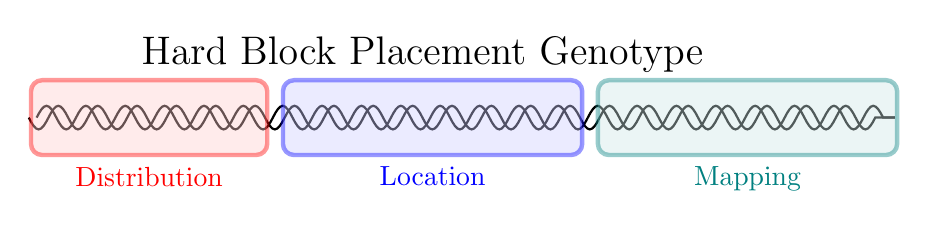
\begin{tikzpicture}[decoration={coil},
dna/.style={decorate, thick, decoration={aspect=0, segment length=0.5cm}}]
 
%DNA
	\draw[dna, decoration={amplitude=.15cm}] (.1,0) -- (11,0);
	\draw[dna, decoration={amplitude=-.15cm}] (0,0) -- (11,0);
	\node at (5,0.8) {\Large Hard Block Placement Genotype};

	\node [rectangle,rounded corners,inner sep=0pt,minimum width=3cm, minimum
  height=0.25cm,text height=0.95cm, draw=red, ultra thick, fill=red!20,
  anchor=west, opacity=0.4, text
  opacity=1,label=below:{\textcolor{red}{Distribution}}] at (0,0) {};

  \node [rectangle,rounded corners,inner sep=0pt,minimum width=3.8cm, minimum
  height=0.25cm,text height=0.95cm, draw=blue, ultra thick, fill=blue!20,
  anchor=west, opacity=0.4, text
  opacity=1,label=below:{\textcolor{blue}{Location}}] at (3.2,0) {};
 

	\node [rectangle,rounded corners,inner sep=0pt,minimum width=3.8cm, minimum
  height=0.25cm,text height=0.95cm, draw=teal, ultra thick, fill=teal!20,
  anchor=west, opacity=0.4, text
  opacity=1,label=below:{\textcolor{teal}{Mapping}}] at (7.2,0) {};
 
	\end{tikzpicture}
	
	}
	
	\subfloat[distribution]{
		\includegraphics[width=0.30\textwidth, valign=t]{figure/geno-distribution.pdf}
		\vphantom{
			\includegraphics[width=0.25\textwidth, valign=t]{figure/geno-location.pdf}
			\includegraphics[width = 0.23\textwidth, valign=t]{figure/geno-mapping.pdf}
		}
	}
	\hfill
	\subfloat[location]{
		\includegraphics[width=0.25\textwidth, valign=t]{figure/geno-location.pdf}
		\vphantom{
			\includegraphics[width = 0.23\textwidth, valign=t]{figure/geno-mapping.pdf}
		}
	}
	\hfill
	\subfloat[mapping]{
		\includegraphics[width = 0.23\textwidth, valign=t]{figure/geno-mapping.pdf}
	}
	
	% \caption{Our three-tier genotype design for hard block placement. 
	% (a) Distribution defines the amount of hard blocks to be placed in each column. 
	% (b) Location encodes the relative position of the corresponding hard blocks in its column. 
	% (c) Mapping defines the connectivity of hard blocks, i.e., which hard blocks are mapped to one convolution unit. 
	% The selected physical hard-block groups are numbered, which corresponds to the mapping genotype.
	% }

	\caption{
		本文提出的“三段”式硬核布局基因型设计。
		(a) Distribution 限定了每一列中选定用于布局的硬核个数;
		(b) Location 限定每一个硬核在该列中的相对位置;
		(c) Mapping 规定了硬核之间的连接关系,也就是逻辑网表中的硬核与FPGA上物理位置的一一对应关系。
	}
	
	

	\label{fig:genotype}
  \vspace{-0.2in}
\end{figure*}

对于以上讨论的布局问题,K个卷积运算单元暴力搜索法需要尝试的问题空间大小在 $SP! \times BRAM! \times URAM! = 9K!\times4K!\times1K!$
的数量级,显然是行不通的。本文提出基于进化算法的应和布局,可以在短时间内发现高质量的布局结果。在进化算法中使用基因型来编码可行解,因此合理的
基因型设计对优化效果有至关重要的影响。我们将布局问题分解为三个子问题:硬核的列分布,硬核在列中的位置,硬核之间的连接关系。根据这三个子问题,我们
设计了对应的基因型。

\begin{itemize}
	\item \textcolor{red}{\bf Distribution} 因为卷积加速器设计中使用的各硬核比例不一定完全符合FPGA板上的硬核资源比例,
		又由于UltraScale系列硬件的硬核资源为按列分布,因此将使用的硬核资源按比例分配到各列,这一部分基因型就是规定了按什么样的比例
		将使用的硬核资源分配到各列。在解码该部分基因型时,首先将其归一化,然后根据归一化后的值和各列含有的硬核数目决定每一列放置
		多少个该种类硬核。
	\item \textcolor{blue}{\bf Location} 在我们决定了每一列放置硬核的数目之后,下一步需要决定的是硬核在每一列中的位置。
		这一部分基因型规定的就是每个硬核在该列的位置。此基因型使用 0$\rightarrow$1 浮点数对应硬核在列中从下到上的相对位置,
		也就是基因型中位置值接近0的硬核将被放置在列下方的位置,接近1的硬核将被放在列上方的位置。
	\item \textcolor{teal}{\bf Mapping} 最终,当确定了硬核放置的数目和位置之后,我们也就确定了在所有的物理硬核位置中,哪些
		硬核位置被选中用于布局。最终需要确定的,是将逻辑网表中的硬核映射到物理位置时候的对应关系。我们将选中的硬核位置编号,
		Mapping基因型中规定这些位置编号的排列,在解码时按顺序将基因型中的排列对应到网表中的硬核,这样就规定了逻辑网表中硬核
		到物理硬核的对应关系。这实际上影响的是每个卷积单元中硬核的连接关系。
\end{itemize}

以上说明的三种子基因型分别对应着布局问题的三个子问题,在图\ref{fig:genotype}中,我们对基因型设计进行了可视化。这三种子基因型
是紧密相关、互相依赖的,因此无法拆解为三个单独的问题分别优化。我们针对这一特性应用 Composite Genotype~\cite{opt4jpaper} 来适应子问题的
依赖关系,具体来说,三个子问题分别编码,在优化过程中分别更新,彼此之间不相互影响,但是在计算基因型的适应度函数 (Fitness Function)
的时候,三个子基因型一同解码计算。


\subsection{基因型解码时的解合法化}

为了适应浮点优化方法,我们通过解合法化 (Solution Legalization) 步骤对基因型采取量化等操作得到实际的布局,这一步骤在解码时进行。
算法 \ref{algo:distribution} 展示了了分布基因型的解码和合法化过程。由于假定可用资源已知,因此我们首先将分布量化为整数,
然后将每个整数值限制到每列的最大可放置硬核数。然后,我们将上一步去掉的硬核均匀分给其他的列。

\begin{algorithm}
	\SetKwFunction{GetDistribution}{GetDistribution}
	\SetKwFunction{Normalize}{Normalize}
	\SetKwFunction{GetMaxBlock}{GetMaxBlock}
	\SetKwFunction{Sum}{Sum}\SetKwFunction{Min}{Min}
	\SetKwFunction{Int}{Int}
	\SetKwInOut{Input}{input}\SetKwInOut{Output}{output}
	
	%\Input{Available hard block resources, distribution genotype}
	%\Output{Number of hard blocks to place for each column}
	%\BlankLine
	hardBlocks = \{DSP48, BRAM, URAM\}\;
	\ForEach {hardBlock in hardBlocks}{
		\tcp{distribution: a float array}
		distribution = \GetDistribution{hardBlock, genotype}\; 
		distribution = \Normalize{Distribution}\;
		\tcp{quantize}
		\For {$i\leftarrow 0$ \KwTo distribution.length}{
			distribution[i] = distribution[i] $\times$ blockSum\;
			distribution[i] = \Min{distribution[i], columnMax}\;
		}
		\tcp{handle rounding error}
		count=0\;
		\While{count $<$ blockSum - \Sum{distribution}}{
			col\_idx = 0\;
			\While{col\_idx $<$ all\_columns}{
				\If{ distribution[col\_idx] + 1 $\leq$ column\_max}{
					distribution[col\_idx] += 1\;
					count++\;
				}
				col\_idx++\;
				\If{count == block\_sum - \Sum{distribution}}{\textbf{break}\;}
			}
		}
		
   }

	\caption{Distribution genotype legalization}
	\label{algo:distribution}
\end{algorithm}

算法 \ref{algo:location} 展示了位置基因型的解码与合法化过程。
由于硬块位置是离散的,因此将对基因型中的连续值进行量化。
每个量化后的值都是级联链中第一个硬核的位置,所以从位置基因型直接解码的级联链位置可能会重叠或超出列中可用的硬核范围。
因此,我们对量化的位置进行排序,并从下至上调整位置。
位置调整首先检查可用的硬核是否足以放置该列剩余的级联链,如果不能则将当前级联链向下调整到所需位置,
来使超出范围的硬核放置合法化。
另一方面,如果当前组与前一组重叠,则将其调整为向上移动,直到合法放置为止。

\begin{algorithm}
	\SetKwFunction{GetLocation}{GetLocation}
	\SetKwFunction{Partition}{Partition}
	\SetKwFunction{Sort}{Sort}
	\SetKwFunction{Int}{Int}
	
	
	hardBlocks = \{DSP48, BRAM, URAM\}\;
	\ForEach {hardBlock in hardBlocks}{
		location = \GetLocation{hardBlock, genotype}\;
		\tcp{partition location into columns}
		location\_columns = \Partition{location, distribution}\;
		\ForEach {l\_column in location\_columns} {
			\Sort{l\_column, ascending}\;
			\For{$i\leftarrow 0$ \KwTo l\_column.length} {
				l\_column[i] $\times$= columnSize\;
				l\_column[i] = \Int{l\_column[i]}\;
				need = (l\_column.length-i-1) $\times$ group\_size\;
				avail = columnSize - (l\_column[i] + group\_size)\;
				\If{need $>$ avail}{l\_column[i] -= need - avail\;}
				\ElseIf{l\_column[i] $<$ l\_column[i-1] + group\_size}{
					l\_column[i] = l\_column[i-1] + group\_size\;
				}
			}
			
			
		}
	}
	
	\caption{Location genotype legalization}	
	\label{algo:location}
\end{algorithm}

由于Mapping基因型只优化编码的顺序,而不对编码的值进行修改,所以不会产生不合法编码,也就不需要解合法化。
以上内容详细阐述了解合法化的步骤,这些步骤保证了布局结果满足三个限制条件,并且与解析布局方法(Analytical Placement)
相比,我们的合法化步骤开销更低。









\section{进化算法:NSGA-II与CMA-ES}

在建立了布局模型的基础上,本节详细阐述本文使用的进化算法优化方法。进化算法用于布局问题的优化相比传统的模拟退火与目前广泛应用的
解析法相比主要有三点优势:(1)与模拟退火相比,进化算法基于种群的优化方式个体之间相互独立,天然具有大规模并行化加速的优势;
(2)多目标遗传算法的发展使得进化算法相比其他方法更擅长优化多个目标函数,在本文中我们利用这一优势设计了两个目标函数分别优化
线长和计算单元限制框,取得了比单目标更好的优化效果;(3)基于概率分布的进化算法在同样的问题规模可以在优化速度和结果质量上同时
超越state-of-the-art的解析布局算法。本节详细介绍RapidLayout布局引擎所使用的两种进化算法:非支配排序遗传算法与协方差矩阵
适应进化策略。

\subsection{非支配排序遗传算法:NSGA-II}

非支配排序遗传算法(Non-Dominated Sorting Genetic Algorithm, NSGA-II~\cite{deb2002fast}) 是一种较早提出的多目标
遗传算法。近年来由于强化学习\cite{li2019deep}和NAS(Neural Architecture Search)\cite{lu2019nsga}中的应用再度流行。
图\ref{fig:NSGA-II}描述了NSGA-II的优化过程,其核心内容是两个排序算法:Non-dominated Sorting 与 Crowd Distance Sorting。

\begin{figure}[h]
	\centering
	\includegraphics[width=0.8\textwidth]{figure/NSGA-II}
	\caption{NSGA-II的优化过程~\cite{deb2002fast}:首先亲代通过交叉变异产生同等数量的子代,然后通过Non-dominated Sorting将种群个体分为
	多个帕累托前端(Pareto-Front),并淘汰一部分劣势个体。如果同一个帕累托前端内的个体需要淘汰,则通过Crowd-Distance Sorting
	保留具有代表性的子代,最终淘汰一半种产生下一代亲代。} 
	\label{fig:NSGA-II}
\end{figure}

{\bf Non-dominated Sorting}
也称为非支配排序方法,是NSGA-II处理多个目标的核心方法,其思想是用“支配”的概念进行排序:如果个体A在各个衡量标准(多个目标函数值)上
均非劣于个体B,则A支配B。在种群中可以根据支配关系将个体分为许多组,每一组内的个体互相不支配,每组内的个体和其他组的个体一定存在支配关系,
这样的组成为帕累托前端(Pareto-Front)。简而言之,因为多目标的存在,在排序过程中只能将个体分为几组,而组内的个体无法直接判断孰优孰劣。
如图\ref{fig:NSGA-II}所示,第一轮淘汰使用的此种排序方法,但如果同一前端需要淘汰部分个体,则需要其他方法。
Non-dominated Sorting的排序算法请见附录\ref{sec:nondominated} 算法 \ref{algo:nondominated}。


{\bf Crowd Distance Sorting}
用于解决同一个帕累托前端内的排序问题。此种排序方法的核心思想是保留同一帕累托前端内部具有“代表性”的个体。
其具体实现方法是首先衡量所有个体在所有目标函数维度上与其邻近的个体之间的距离,根据距离首先计算出所有点的 crowd distance 值,
其具体做法于附录\ref{sec:crowd}算法 \ref{algo:crowd-distance-assign}中详细说明。然后根据 crowd distance排序,
最终与其邻近个体在所有目标函数维度上距离小的被淘汰,距离大的被保留,也就是保留了具有“代表性”的个体,实际此种排序淘汰算法促使
种群个体在所有目标函数维度上均匀分布。
Crowd Distance Sorting的排序算法请见附录\ref{sec:crowd} 算法 \ref{algo:crowd-distance-sorting}。



\subsection{协方差矩阵适应进化策略:CMA-ES}

协方差矩阵适应进化策略(Covariance Matrix Adapted Evolution Strategy, CMA-ES) 是实数域上的一种优化方法,
适合于黑箱问题、非线性优化、病态(ill-conditioned)系统优化,并且无需导数\cite{cmapaper}。CMA-ES是一种
state-of-the-art的进化算法,被用于包括神经网络参数优化\cite{nn2016cma}在内的多个领域。
CMA-ES无需求导的特性使其适用于许多gradient-based方法失败的问题,或一些非平滑,非连续域的优化问题。
CMA-ES将产生可行解的过程建模为均值向量为$\mathbf{\mu}$,协方差矩阵为 $\mathbf{C_{\sigma}}$的高斯随机过程
采样。在每次进化过程中新的可行解使用更新后的均值向量和协方差矩阵采样得到,然后根据目标函数对可行解进行排序,
最后使用前25\%的可行解更新均值向量与协方差矩阵。算法\ref{algo:cma}详细描述了CMA-ES的实现原理和参数设置。

{\bf 参数设置:}

$\lambda = 4 + \lfloor 3 ln(n) \rfloor$, $\mu = \lfloor \lambda / 2\rfloor$,
$w_i = \frac{ln(\mu+1) - ln(i) }{\sum_{j=1}^{\mu}ln(\mu+1)-ln(j) } \ (i=1,...,\mu) $, 
$\mu_w = \frac{1}{\sum_{i=1}^{\mu} w_i^2}$, 
$c_\sigma = \frac{\mu_w + 2}{n + \mu_w + 3}$,
$d_\sigma =  1 + 2 max (0, \sqrt{\frac{\mu_w-1}{n+1}-1} + c_\sigma)$,
$c_c = \frac{4}{n+4}$, $\mu_{cov} = \mu_w$, 
$c_{cov} = c_{cov}^{def} = \frac{1}{\mu_{cov}} \frac{2}{(n+\sqrt{2})^2} + (1 - 1/\mu_{cov}) min (1, \frac{2\mu_{cov}-1}{(n+2)^2+\mu_cov})$


{\bf 参数初始化:}

$g=0$, $\mathbf{B=I}$, $\mathbf{D=I}$, $\mathbf{p_\sigma=(0,..,0)^T}$,
$\mathbf{p_c} = (0,...,0)^T$, $\mathbf{C=I}$, $\langle x \rangle_w \in \mathbb(R)^n$,
$\sigma \in \mathbf{R}$


\begin{algorithm}
	\SetKwFunction{eigendecomposition}{eigendecomposition}
	\SetKwFunction{exp}{exp}

	\While{Stop Criterion not Reached}{
		$g \leftarrow g + 1$

		$z_i \sim \mathcal{N}(0,\, \mathbf{I}) \  for \  i = 1,...,\lambda$

		$x_i = \langle x \rangle_w + \sigma\mathbf{BDz_i}$
		
		$\langle x \rangle_w = \sum_{i=1}^{\mu} w_i\mathbf{x_{i:\lambda}}$ \tcp*{$\mathbf{x_{i:\lambda}}$ denotes the $i$-th best individual out of the $\lambda$}

		$\langle z \rangle_w = \sum_{i=1}^{\mu} w_i\mathbf{z_{i:\lambda}}$ \tcp*{$\mathbf{z_{i:\lambda}}$ denotes the $i$-th best mutation vector}

		$\mathbf{p_\sigma} \leftarrow (1-c_\sigma)\mathbf{p_\sigma} + \sqrt{c_{\sigma}(2-c_{\sigma})} \sqrt{\mu_w}\mathbf{B} \langle z \rangle_w$
		
		\If{ $\|\mathbf{p_\sigma}\| / \sqrt{1-(1-c_\sigma)^{2g}} < (1.4 + 2/(n+1)) E(\|\mathcal{N}(0,\, \mathbf{I})\|)$ }{
			$H_\sigma = 1$
		}
		\Else {
			$H_\sigma = 0$
		}

		$\mathbf{p_c} \leftarrow (1-c_c)\mathbf{p_c} + H_\sigma \sqrt{c_c(w-c_c)}\sqrt{\mu_w}\mathbf{BD\langle z \rangle_w}$

		$\mathbf{C} \leftarrow (1-c_{cov} \mathbf{C}) + 1/\mu_{cov}c_{cov}\mathbf{p_c{p_c}^T} + c_{cov}(1-1/\mu_{cov})\sum_{i=1}^{\mu}w_i\mathbf{BDz_{i:\lambda}(BDz_{i:\lambda})^T}$

		$\sigma \leftarrow \sigma $ exp($c_\sigma / d_\sigma (\|\mathbf{p_\sigma]}\|/E(\|\mathcal{N}(0,\, \mathbf{I})\|)) - 1$)

		$\mathbf{B\,D^2} =$ eigendecomposition($\mathbf{C}$)
		
	}
	
	\caption{The $(\mu/\mu_W, \lambda)$ CMA-ES Algorithm}	
	\label{algo:cma}
\end{algorithm}

为了适应大规模优化问题,本文修改了协方差矩阵的更新方法\cite{large-scale-cma},
令 $\mathbf{D^2}=diag(\mathbf{C})$, $c_{cov} = \frac{n+2}{3}c_{cov}^{def}$,
也就是将协方差矩阵的更新限制在对角线,其余元素置零,并提高了学习率。这种优化方法使得
CMA-ES的空间复杂度由二次减低为线性,加快了大规模问题的优化速度。



\section{RapidLayout布局框架}

上一节详细阐述了布局问题的建模、目标函数、优化限制,以及本文提出的进化算法基因型设计、解合法化步骤。在此基础上,
我们基于Xilinx RapidWright FPGA 实现框架设计并且实现了端到端的布局布线框架,RapidLayout。RapidLayout
的核心部分是上一节中描述的进化算法布局引擎,此小结中详细阐述RapidLayout的设计工作流程,各实现步骤的含义,
内容,及实现方法。图\ref{fig:flow}展示了RapidLayout的工作流。


% figure: design flow

\tikzstyle{block} = [thick, rectangle, draw, fill=white, text width=12em, text centered, rounded corners, minimum height=2em]
\tikzstyle{invisiblock} = [rectangle, fill=white, text width=12em, text centered, rounded corners, minimum height=2em]
\tikzstyle{decisionblock} = [rectangle, draw, fill=blue!20, text width=12em, text centered, rounded corners, minimum height=2em]
\tikzstyle{line} = [draw, -latex']


\pgfdeclarelayer{bg}    % declare background layer
\pgfsetlayers{bg,main}  % set the order of the layers (main is the standard layer)


\begin{figure}
 \begin{center}
 \begin{tikzpicture}[node distance=1.5cm and 3.5cm, scale=1, transform shape]
   % Place nodes
   \node [invisiblock] (input) {Convolution Block DCP};
   \node [block, below of=input] (replicate) {Netlist Replication {\bf [\textless 1s]}};
   \circledat{A}{replicate.north west};
   \node [block, below of=replicate, minimum height=7em, node distance=2.5cm] (evolve) {Evolutionary\\ Hard Block\\ Placement\\ {\bf [30\,s--5\,min]}};
   \circledat{B}{evolve.north west};
   \node [block, below of=evolve, node distance=2.5cm] (siteroute) {Placement and\\ Site Routing {\bf [$\approx$3\,min]}};
   \circledat{C}{siteroute.north west};
   \node [block, below of=siteroute] (pipeline) {Post-Placement\\Pipelining {\bf [$\approx$10\,s]}};
   \circledat{D}{pipeline.north west};
   \node [block, below=0.75cm of pipeline] (vivado) {SLR Placement\\ and Routing {\bf [$\approx$54\,min]}};
   \circledat{E}{vivado.north west};
   \node [block, below=0.75cm of vivado] (slr) {SLR Replication {\bf [$\approx$2\,min]}};
   \circledat{F}{slr.north west};
   % Draw sub-nodes
  	 \node [block, fill=teal!50, right=1cm of evolve] (two) {Compute objective};
   \node [block, fill=teal!50, above of=two] (one) {Generate candidates};
   \node [block, fill=teal!50, below of=two] (three) {Update};
   % Inner loop highlight
   \begin{pgfonlayer}{bg}
   
   \path[rounded corners, draw=blue, thick, fill=blue!10,opacity=0.9] 
	([xshift=-0.75em,yshift=0.75em]vivado.north west) to ([xshift=10em,yshift=0.75em]vivado.north east) 
	to ([xshift=10em,yshift=-0.75em]vivado.south east) to ([xshift=-0.75em,yshift=-0.75em]vivado.south west) -- cycle;
   
   
   \path[rounded corners, draw=red, thick, fill=red!10,opacity=0.9] 
	([xshift=-0.75em,yshift=0.75em]replicate.north west) to 
 ([xshift=20em,yshift=0.75em]replicate.north east) to 
 ([xshift=20em,yshift=-0.75em]slr.south east) to
 ([xshift=-0.75em,yshift=-0.75em]slr.south west) to
 ([xshift=-0.75em,yshift=0.75em]slr.north west) to 
 ([xshift=12em,yshift=0.75em]slr.north east) to
	([xshift=12em,yshift=-0.75em]pipeline.south east) to 
 ([xshift=-0.75em,yshift=-0.75em]pipeline.south west) -- cycle;
   
   \path[rounded corners, draw=teal, thick, fill=teal!10,opacity=0.9] 
	([xshift=-0.5em,yshift=0.5em]evolve.north west) to ([xshift=0.5em,yshift=0.5em]evolve.north east) 
	to ([xshift=-0.5em,yshift=1.5em]one.north west) to ([xshift=3.5em,yshift=1.5em]one.north east) 
	to ([xshift=3.5em,yshift=-1.5em]three.south east) to ([xshift=-0.5em,yshift=-1.5em]three.south west) 
	to ([xshift=0.5em,yshift=-0.5em]evolve.south east) to ([xshift=-0.5em,yshift=-0.5em]evolve.south west) -- cycle;
   \end{pgfonlayer}
   
   %\node [draw=none,below right=0.1cm of three] (opt4j) {\bf Opt4J};
   \node [draw=none,right=3.5cm of slr] (RapidWright) {\Large \bf RapidWright};
   \node [draw=none,right=1.75cm of vivado] (RapidWright) {\Large \bf Vivado};
   
   \node [invisiblock,below of=slr] (output) {Bitstream};
   % Draw edges
   \path [line, thick] (input) -- (replicate);
   \path [line, thick] (replicate) -- (evolve);
   \path [line, thick] (evolve) -- (siteroute);
   \path [line, thick] (siteroute) -- (pipeline);
   \path [line, thick] (pipeline) -- (vivado);
   \path [line, thick] (vivado) -- (slr);
   \path [line, thick] (slr) -- (output);
   % Draw sub-edges
   \path [line, thick] (one) -- (two);
   \path [line, thick] (two) -- (three);
   % Loops
   \path [line, thick] (three.east) -- ([xshift=0.8cm]three.east) -- ([xshift=0.8cm]one.east) node [midway, above, sloped, rotate=180] (textnode0) {evolve} -- (one.east);

 \end{tikzpicture}
 \end{center}
% 	\caption{RapidLayout Design Flow with runtime details for the Xilinx VU11P
%  FPGA along with tool usage information. Bulk of the intelligent exploration is done in RapidWright, and Vivado is only invoked at the end for final placement and routing.}
 
 \caption{RapidLayout工作流,以Xilinx VU11P FPGA上的实现流程为例。主要的布局优化和物理实现工作由RapidWright API开发完成,Vivado只负责
 控制逻辑布局以及SLR内的布线。}
 
 \label{fig:flow}
 \vspace{-0.1in}
\end{figure}


\circled{A} {\bf 逻辑网表复制}
RapidLayout的输入是一个卷积计算单元的逻辑网表,以一个DCP checkpoint 文件的形式存储。RapidLayout首先根据选定的FPGA器件型号
和卷积计算单元内的各硬核比例计算出{\bf 最小可复制矩形域(Minimum Replicating Rectangle)} 同时确定矩形域最大可放置的卷积单
元个数。最小可复制矩形域是进行布局方案优化的区域,其具体含义为:根据设计使用的硬核比例与物理硬核资源比例确定的最小矩形,在此矩形内
可使各硬核利用率达到最高,同时其布局结果可用于复制填充至整个FPGA。确定布局范围以及该范围内卷积计算单元个数之后,RapidLayout复制
输入的逻辑网表并连接全局信号(reset, clock等)。以VU11P FPGA为例,RapidLayout确定的最小可复制矩形范围是宽为8个时钟域,高为2
个时钟域,可放置80个卷积运算单元,三种硬核的利用率均在95\%以上。这一最小可复制矩形区域内的布局结果可经过2次复制充满一个超逻辑域,
可经过6次复制充满整个FPGA。

\circled{B} {\bf 基于进化算法硬核布局}
RapidLayout使用非支配排序遗传算法(Non-Dominated Sorting Genetic Algorithm II, NSGA-II) 或协方差矩阵适应进化策略
(Covariance Matrix Adapted Evolution Strategy, CMA-ES) 两种进化算法对硬核布局优化。进化算法包括产生可行解,计算适应
度,更新可行解等操作,在计算适应度的步骤需要根据布局方法计算线长。由于进化算法是一种重复优化方法(Iterative Method),所以
我们不可能依赖Vivado估计每一个可行解的线长,否则会需要依次进行物理布局,导致优化时间过长。RapidWright的优势在于可以快速获得
FPGA的物理信息,因此本文利用Rapidwright快速计算出板上物理位置之间布线所需的线长。

\circled{C} {\bf 物理网表布局和Site布线}
优化过程结束,RapidLayout会得到最小可复制矩形内的最优布局结果。然后根据这一结果将逻辑网表和布局结果复制到整个超逻辑域(SLR),
再修改物理网表,进行实际的物理布局操作。本文使用RapidWright提供的FPGA物理层API开发了三种硬核的布局方法,首先将硬核放置在对
应的物理位置(Site),然后进行“Site 布线”,连接硬核与Site内部的信号接口,这一步骤保证了布局之后导出的DCP checkpoint文件
与Vivado的兼容性。

\circled{D} {\bf 流水线}
布局完成之后,硬核的物理位置已经确定,因此可以估计硬核之间的布线线长和需要插入的寄存器个数,对较长的数据通路进行流水线,以得到
较高的时钟频率。这个步骤在布局之后进行,是为了保证正确的数据通路插入合适的寄存器个数。进行流水线操作的目的是为了让整个加速器设
计的时钟频率达到650MHz以上。650MHz是脉动阵列中Ultra RAM运行的上限,通过流水线插入寄存器的方式我们可以获得高于650MHz的时钟频率,但
实际运行中的时钟还是需要设置在650MHz。此步骤在URAM $\rightarrow$ BRAM 和 BRAM $\rightarrow$ DSP 之间的数据通路插入
流水线寄存器,数目根据线长确定。

\circled{E} {\bf 超逻辑域布局与布线}
RapidLayout负责完成硬核布局布线,控制逻辑和流水线寄存器等使用的LUT和Flip-Flop则又Vivado完成布局和布线。在此步骤中,流水线
之后的设计首先被导出成DCP checkpoint文件,然后由Vivado读入完成超逻辑域的布局与布线,完成布局布线的设计也以DCP checkpoint
的形式存储。

\circled{F} {\bf 超逻辑域复制}
在上一步步骤中RapidLayout完成了单个超逻辑域的完整实现,以VU11P为例整个FPGA中有3个超逻辑域,每个超逻辑域内部的器件构造与排布
相同。因此,我们使用RapidWright的硬件API开发了SLR复制的功能,将一个SLR的布局布线结果连同逻辑网表复制到整个FPGA的所有超逻辑域,
由此获得了大幅的时间节省。

对于VU11P FPGA来说,RapidLayout 端到端的工作流与Vivado的实现工作流相比要快$\approx$5--6$\times$。RapidLayout的整个工作流
仅需大约1小时,并且无需输入手工布局信息,整个流程自动化;Vivado则需要以XDC Constraints的方式输入手工完成的硬核布局,否则其布局引擎
无法产生可布线的结果,并且整个工作流耗费5--6小时。手工的硬核布局需要经验和长达几周的反复调试才能使时钟频率达到650MHz以上,而RapidLayout
使用进化算法布局引擎可以在几分钟的时间内自动发现高质量的硬核布局结果,无需手动调试和先前经验。


\section{RapidLayout以Xilinx VU11P FPGA为例的布局实现过程}
\label{sec:visual}

上一节介绍了RapidLayout布局框架的工作流,本节以Xilinx UltraScale+ VU11P FPGA的实现为例阐述布局的三个过程,从单个卷积运算单元
的布局到整个FPGA的完全实现。


\begin{figure}
\centering
\includegraphics[width=0.5\textwidth, valign=c]{figure/block1.pdf}
% \caption{Floorplan layout visualization of a single convolution block
% implementation supporting dual 3$\times$3 kernels to match URAM bandwidth. This
% is the design shown in Figure~\ref{fig:RTL} earlier. The
% bounding polygon that encloses all hard blocks and the routing connections is
% shown in gray.}
\caption{一个卷积计算单元的布局结果可视化。此卷积计算单元的RTL设计如图ref{fig:sys}所示。其中
布局使用的硬核高亮标出,整体的布线范围使用灰色阴影区域标出}
\label{fig:block1}	
\end{figure}

\begin{figure}
\centering
\includegraphics[width=0.8\textwidth, valign=c]{figure/block80.pdf}
% \caption{Floorplan layout visualization of a single repeating rectangular region
%  layout with 80 convolution blocks. The bounding polygon from
% Figure~\ref{fig:block1} is also shown here for scale.}
\caption{最小可复制矩形区域内的布局结果可视化。此最小可复制矩形域放置了80个卷积计算单元,图\ref{fig:block1}的
位置在图中标出用作比例参考}
\label{fig:block80}	
\end{figure}


{\bf 单个卷积运算单元的布局:} 图\ref{fig:block1}展示了单个卷积运算单元的布局结果。本文为硬核布局设计了一套可视化套件,包含在
RapidLayout框架中,包含单个卷积单元的位置信息、整体的布局可视化结果、以及布局过程的动态展示。图中浅色矩形为三种硬核的分布列,其中
被选中的硬核位置被高亮标出,整个卷积核的分布范围使用灰色阴影标出。从图中可以发现,URAM、BRAM、DSP资源列分布不规则,这导致了单个
卷积运算单元的布局不规则,也说明了单个卷积单元的布局结果无法直接通过复制-粘贴 (\textit{copy-paste}) 的方式适用于所有卷积单元。

{\bf 一个最小可复制矩形区域:} RapidLayout根据器件型号和设计中使用硬核的比例自动确定最小可复制矩形区域,最大化每种硬核的使用率来
得到最高的计算密度,同时便于布局结果复用,最小化优化问题规模从而加快速度。在图\ref{fig:block80}中展示了VU11P FPGA 最小可复制
矩形区域内的布局结果,使用与图\ref{fig:block1}相同的可视化方法。该最小可复制矩形区域宽8个时钟域、高2个时钟域,放置了80个卷积运算
单元,URAM利用率100\%,DSP48利用率93.7\%,BRAM利用率95.2\%,完整FPGA实现的硬核利用率与此相同。从图中的灰色重叠区域将
可以观察到阻塞(Congestion)情况,RapidLayout的布局引擎可以最小化重叠,从而减小布线资源的阻塞。

{\bf 完整FPGA实现:} 图\ref{fig:fullchip}展示了RapidLayout从最小可复制矩形区域的布线出发完成整个FPGA布线的步骤。首先RapidLayout
将最小区域内的布线结果复用,复制粘贴直到布满一个超逻辑域,在VU11P上则是复制2次充满了SLR0。随后,RapidLayout调用Vivado完成
控制逻辑的布局与完整布线,得到了一个超逻辑域(SLR0)的完整实现。下一步,RapidLayout将一个超逻辑域(SLR0)内部的完整实现通过
复制粘贴的方式复用到其他超逻辑域(SLR1, SLR2)上,得到完整的FPGA实现,可产生比特流。



\begin{figure}
\centering	
\scalebox{1.2}{%
 \begin{tikzpicture}
 \centering
   \pgftext{%
     \includegraphics[width=0.26\textwidth]{figure/rapidlayout-placed.png}
   }%
   \node [rectangle,rounded corners,minimum width=4cm,minimum
   height=0.7cm,draw=green,ultra thick,anchor=south west] (rect1) at
   (0.1-2.2,0.75-2.25) {};
   \node [rectangle,rounded corners,minimum width=4.2cm,minimum
   height=1.5cm,draw=red,ultra thick,anchor=south west,
   text=white,text opacity=0.5] (slr0) at
   (0-2.2,0-2.25) {\Huge SLR0};
   \node [rectangle,rounded corners,minimum width=4cm,minimum
   height=0.7cm,fill=green,opacity=0.5,draw
   opacity=1,draw=green,ultra thick,anchor=south
   west,text=black,text opacity=1,align=center] (rect0) at
   (0.1-2.2,-2.25+0.05) {Repeat Rect. (Fig~\ref{fig:block80})};
   \node [rectangle,rounded corners,minimum width=4.2cm,minimum
   height=1.5cm,draw=red,ultra thick,anchor=south west,
   text=white,text opacity=0.5] (slr1) at
   (0-2.2,1.5-2.25) {\Huge SLR1};
   \node [rectangle,rounded corners,minimum width=4.2cm,minimum
   height=1.5cm,draw=red,ultra thick,anchor=south west,
   text=white,text opacity=0.5] (slr2) at
   (0-2.2,3-2.25) {\Huge SLR2};
   \draw [ultra thick,->,green] (rect0) to [out=0,in=0,looseness=2] node (b)
 [midway,above=0cm,align=center,rotate=-90] {\textcolor{green}{Copy Placements +
 }\\\textcolor{green}{Vivado P+R}} (rect1);
 \draw [ultra thick,->,red] (slr0) to [out=180,in=180] node (a)
 [midway,above,align=center,rotate=90] {\textcolor{red}{Copy Placement +
 Routing}\\\textcolor{red}{in RapidWright}} (slr2);
   \circledat{F}{[yshift=2cm,xshift=0.35cm]a};
   \circledat{C}{[yshift=1cm,xshift=0.75cm]b};
   \circledat{D}{[yshift=0.0cm,xshift=0.75cm]b};
   \circledat{E}{[yshift=-1cm,xshift=0.75cm]b};
   \draw [ultra thick,->,red] (slr0) to [out=180,in=180] (slr1);
 \end{tikzpicture}
}
%  \caption{Full-chip layout for the systolic array accelerator generated from a
% repeating rectangle of size two clock regions high and the full chip wide. After
% one replication we span one SLR region. We place and route this with Vivado,
% export DCP, reimport into RapidWright to clone across SLRs.}

\caption{从最小可重复矩形区域内的布局结果到完整FPGA实现过程示意图。首先,最小可重复
矩形内的布局结果经过一次复制充满SLR0,RapidLayout对布局结果和逻辑网表同时进行复制。然后RapidLayout调用Vivado完成SLR0
的布局布线,得到SLR0的完整实现。最后,RapidLayout使用RapidWright API将SLR0的布局结果和布线结果复用到
SLR1和SLR2,得到完整的FPGA实现。}
 \label{fig:fullchip}

\end{figure}














\section{本章小结}

本章首先介绍了硬核布局建模为多目标优化问题的方法,明确了问题的优化目标与限制,阐述了本文的创新基因型设计与相应的
解合法化过程,明确NSGA-II与CMA-ES的算法原理与实现方案,最终介绍了RapidLayout布局框架的工作流,并
以层层递进的方式举例阐述了脉动阵列的布局实现过程。














































% \chapter{几何驱动的用户目标区域提取与矫正方法}
% 内容概括 \cite{zhang98}。

% \section{勾画式用户目标区域标注}
% 勾画式用户标注,是一种简单易行的标注方法\cite{hariharan14,Li08,Su81,Liu93,jiang99} 。……

% \section{基于颜色聚类的目标区域提取方法}
% \label{sec1}
% 这里的颜色分类其实是为图像目标区域提取服务的。通过对图像颜色进行分类,结合用户的标注指定,我们得到用户期望的目标区域的颜色分类,根据这些分类就能够提取出颜色传递的目标区域。……

% \section{几何驱动的目标区域边界矫正方法}
% \ref{sec1} 节提出的目标区域提取方法可以在均匀性或一致性的前提下将图像目标物体或目标区域分割出来,若与相邻部分合并则会破坏这种一致性。

% \section{几何驱动的目标区域提取与矫正实验结果分析}
% 我们进行了图像目标区域提取与矫正实验。……

% \section{本章小结}
% 本章阐述了图像局部颜色编辑方法中图像目标区域提取的相关方法,……
